\documentclass[12pt]{article}
\usepackage{latexblog}

% ============================================================
% Blog Metadata
% ============================================================
\blogtitle{创建一个Flutter的插件}
\blogdate{2019-05-13}
\blogtags{Android, Flutter, 移动端, 闲话编程}
\bloglang{zh}
\blogsummary{}

\begin{document}
\makeblogtitle

最近需要在Flutter中实现AES加解密和KDF，但搜索了一下貌似网络上没有现成的库可以用，因此尝试手写了一个Flutter的插件，实现两个功能：

\begin{itemize}
\tightlist
\item
  AES256/CBC/NoPadding 加解密
\item
  Argon2（Argon2d)
\end{itemize}

\section{插件定义}\label{ux63d2ux4ef6ux5b9aux4e49}

\subsection{创建插件工程}\label{ux521bux5efaux63d2ux4ef6ux5de5ux7a0b}

其实貌似也可以在Flutter项目中直接调用Platform channel相关的实现，考虑到把这一部分剥离出来可以单独维护和造福后人，还是选择创建一个Plugin。首先需要创建一个插件的工程，通过如下的命令：

\begin{Shaded}
\begin{Highlighting}[]
\ExtensionTok{flutter}\NormalTok{ create }\AttributeTok{{-}{-}org}\NormalTok{ com.riguz }\AttributeTok{{-}{-}template}\OperatorTok{=}\NormalTok{plugin encryptions}
\end{Highlighting}
\end{Shaded}

这样会生成一个项目，值得注意的是，这里Android会使用Java，IOS会使用Objective-C。但Objective-C对于我这种没有基础的人来说看着太麻烦了，我尝试了一些之后放弃了。于是需要切换成Swift。这里有一个小的方法可以只修改IOS的部分：

\begin{Shaded}
\begin{Highlighting}[]
\BuiltInTok{cd}\NormalTok{ encryptions}
\FunctionTok{rm} \AttributeTok{{-}rf}\NormalTok{ ios examples/ios}
\ExtensionTok{flutter}\NormalTok{ create }\AttributeTok{{-}i}\NormalTok{ swift }\AttributeTok{{-}{-}org}\NormalTok{ com.riguz .}
\end{Highlighting}
\end{Shaded}

删除ios的目录后执行这个命令，可以重新生成ios的工程，基于swift的。

\subsection{定义Dart接口}\label{ux5b9aux4e49dartux63a5ux53e3}

首先定义出我们要暴露的接口。举个例子，对于AES加密的函数，我们可以这样写：

\begin{Shaded}
\begin{Highlighting}[]
\KeywordTok{class}\NormalTok{ Encryptions }\OperatorTok{\{}
  \AttributeTok{static} \AttributeTok{const}\NormalTok{ MethodChannel \_channel }\OperatorTok{=} \AttributeTok{const}\NormalTok{ MethodChannel(}\StringTok{\textquotesingle{}encryptions\textquotesingle{}}\NormalTok{);}

  \AttributeTok{static} \DataTypeTok{Future}\OperatorTok{\textless{}}\NormalTok{Uint8List}\OperatorTok{\textgreater{}}\NormalTok{ aesEncrypt(}
\NormalTok{      Uint8List key}\OperatorTok{,}\NormalTok{ Uint8List iv}\OperatorTok{,}\NormalTok{ Uint8List value) }\AttributeTok{async} \OperatorTok{\{}
    \KeywordTok{return} \AttributeTok{await}\NormalTok{ \_channel}
        \OperatorTok{.}\NormalTok{invokeMethod(}\StringTok{"aesEncrypt"}\OperatorTok{,} \OperatorTok{\{}\StringTok{"key"}\OperatorTok{:}\NormalTok{ key}\OperatorTok{,} \StringTok{"iv"}\OperatorTok{:}\NormalTok{ iv}\OperatorTok{,} \StringTok{"value"}\OperatorTok{:}\NormalTok{ value}\OperatorTok{\}}\NormalTok{);}
  \OperatorTok{\}}
\end{Highlighting}
\end{Shaded}

这里有几点值得注意的：

\begin{itemize}
\tightlist
\item
  MethodChannel是用来调用原生接口，后面各个平台会注册同名的MethodChannel。
\item
  调用原生方法通过方法名 + 参数调用，参数的对应列表参见官方文档。这里我们希望的是Java中的byte{[}{]} 类型，所以用Uint8List
\item
  参数通过key-value的map传递到原生接口，原生代码通过参数名取得参数值
\end{itemize}

\section{Platform实现}\label{platformux5b9eux73b0}

\subsection{ios}\label{ios}

首先需要先build一下:

\begin{Shaded}
\begin{Highlighting}[]
\BuiltInTok{cd}\NormalTok{ encryptions/example}\KeywordTok{;} \ExtensionTok{flutter}\NormalTok{ build ios }\AttributeTok{{-}{-}no{-}codesign}
\end{Highlighting}
\end{Shaded}

在Xcode中打开项目，有一个SwiftEncryptionsPlugin的类，在这个里面实现即可：

\begin{Shaded}
\begin{Highlighting}[]
\KeywordTok{public} \KeywordTok{func} \FunctionTok{handle}\OperatorTok{(}\VariableTok{\_} \VariableTok{call}\OperatorTok{:} \DataTypeTok{FlutterMethodCall}\OperatorTok{,} \VariableTok{result}\OperatorTok{:}\NormalTok{ @}\DataTypeTok{escaping} \VariableTok{FlutterResult}\OperatorTok{)} \OperatorTok{\{}
    \KeywordTok{let} \VariableTok{args} \OperatorTok{=}\NormalTok{ call}\OperatorTok{.}\NormalTok{arguments }\KeywordTok{as}\OperatorTok{!} \OperatorTok{[}\NormalTok{String}\OperatorTok{:}\NormalTok{ Any}\OperatorTok{];}
    \ControlFlowTok{switch}\NormalTok{ call}\OperatorTok{.}\NormalTok{method }\OperatorTok{\{}
    \ControlFlowTok{case} \StringTok{"aesEncrypt"}\OperatorTok{,} \StringTok{"aesDecrypt"}\OperatorTok{:}
        \KeywordTok{let} \VariableTok{key} \OperatorTok{=}\NormalTok{ args}\OperatorTok{[}\StringTok{"key"}\OperatorTok{]} \KeywordTok{as}\OperatorTok{!}\NormalTok{ FlutterStandardTypedData}\OperatorTok{;}
        \KeywordTok{let} \VariableTok{iv} \OperatorTok{=}\NormalTok{ args}\OperatorTok{[}\StringTok{"iv"}\OperatorTok{]} \KeywordTok{as}\OperatorTok{!}\NormalTok{ FlutterStandardTypedData}\OperatorTok{;}
        \KeywordTok{let} \VariableTok{value} \OperatorTok{=}\NormalTok{ args}\OperatorTok{[}\StringTok{"value"}\OperatorTok{]} \KeywordTok{as}\OperatorTok{!}\NormalTok{ FlutterStandardTypedData}\OperatorTok{;}
        
        \ControlFlowTok{do} \OperatorTok{\{}
            \KeywordTok{let} \VariableTok{cipher} \OperatorTok{=} \ControlFlowTok{try}\NormalTok{ handleAes}\OperatorTok{(}\NormalTok{key}\OperatorTok{:}\NormalTok{ key}\OperatorTok{.}\NormalTok{data}\OperatorTok{,}\NormalTok{ iv}\OperatorTok{:}\NormalTok{ iv}\OperatorTok{.}\NormalTok{data}\OperatorTok{,}\NormalTok{ value}\OperatorTok{:}\NormalTok{ value}\OperatorTok{.}\NormalTok{data}\OperatorTok{,}\NormalTok{ method}\OperatorTok{:}\NormalTok{ call}\OperatorTok{.}\NormalTok{method}\OperatorTok{);}
\NormalTok{            result}\OperatorTok{(}\NormalTok{cipher}\OperatorTok{);}
        \OperatorTok{\}} \ControlFlowTok{catch} \OperatorTok{\{}
\NormalTok{            result}\OperatorTok{(}\KeywordTok{nil}\OperatorTok{);}
        \OperatorTok{\};}     
        \CommentTok{// ...}
    \OperatorTok{\}}
\OperatorTok{\}}
\end{Highlighting}
\end{Shaded}

因为需要使用Argon2，需要在swift中调用原生c代码，试了一些办法都不行，后来发现其实比较简单，直接在Supported Files中有一个encryptions-umbrella.h文件中加入引用，就可以直接调用了:

\begin{Shaded}
\begin{Highlighting}[]
\PreprocessorTok{\#}\ErrorTok{import "EncryptionsPlugin.h"}
\PreprocessorTok{\#}\ErrorTok{import "argon2.h"}
\end{Highlighting}
\end{Shaded}

\begin{Shaded}
\begin{Highlighting}[]
\KeywordTok{func} \FunctionTok{argon2i}\OperatorTok{(}\VariableTok{password}\OperatorTok{:} \DataTypeTok{Data}\OperatorTok{,} \VariableTok{salt}\OperatorTok{:} \DataTypeTok{Data}\OperatorTok{)}\NormalTok{{-}\textgreater{} }\FunctionTok{Data} \OperatorTok{\{}
    \KeywordTok{var} \VariableTok{outputBytes}  \OperatorTok{=} \OperatorTok{[}\NormalTok{UInt8}\OperatorTok{](}\NormalTok{repeating}\OperatorTok{:} \DecValTok{0}\OperatorTok{,}\NormalTok{ count}\OperatorTok{:}\NormalTok{ hashLength}\OperatorTok{);}
    
\NormalTok{    password}\OperatorTok{.}\NormalTok{withUnsafeBytes }\OperatorTok{\{}\NormalTok{ passwordBytes }\ControlFlowTok{in}
\NormalTok{        salt}\OperatorTok{.}\NormalTok{withUnsafeBytes }\OperatorTok{\{}
\NormalTok{            saltBytes }\ControlFlowTok{in}
\NormalTok{            argon2i\_hash\_raw}\OperatorTok{(}\NormalTok{iterations}\OperatorTok{,}\NormalTok{ memory}\OperatorTok{,}\NormalTok{ parallelism}\OperatorTok{,}\NormalTok{ passwordBytes}\OperatorTok{,}\NormalTok{ password}\OperatorTok{.}\NormalTok{count}\OperatorTok{,}\NormalTok{ saltBytes}\OperatorTok{,}\NormalTok{ salt}\OperatorTok{.}\NormalTok{count}\OperatorTok{,} \OperatorTok{\&}\NormalTok{outputBytes}\OperatorTok{,}\NormalTok{ hashLength}\OperatorTok{);}
        \OperatorTok{\}}
    \OperatorTok{\}}
    
    \KeywordTok{return}\NormalTok{ Data}\OperatorTok{(}\NormalTok{bytes}\OperatorTok{:}\NormalTok{ UnsafePointer}\OperatorTok{\textless{}}\NormalTok{UInt8}\OperatorTok{\textgreater{}(}\NormalTok{outputBytes}\OperatorTok{),}\NormalTok{ count}\OperatorTok{:}\NormalTok{ hashLength}\OperatorTok{);}
\OperatorTok{\}}
\end{Highlighting}
\end{Shaded}

\subsection{Android}\label{android}

在Android Studio中打开工程（第一次打开是需要build的，\texttt{cd\ encryptions/example;\ flutter\ build\ apk}， ios也类似）。Android中实现起来会简单一点，这里只说一下如何调用c原生代码：

首先在build.gradle中加入额外的步骤：

\begin{Shaded}
\begin{Highlighting}[]
\NormalTok{externalNativeBuild }\OperatorTok{\{}
\NormalTok{    cmake }\OperatorTok{\{}
\NormalTok{        path }\StringTok{"src/main/cpp/CMakeLists.txt"}
    \OperatorTok{\}}
\OperatorTok{\}}
\end{Highlighting}
\end{Shaded}

然后在CMakeLists.txt中指定编译步骤，我这里需要编译一个argon2的库，以及一个JNI调用的库。

\begin{Shaded}
\begin{Highlighting}[]
\KeywordTok{add\_library}\NormalTok{(}
        \BaseNTok{argon2}
        \OtherTok{SHARED}

\NormalTok{        argon2/src/argon2.c}
\NormalTok{        argon2/src/core.c}
\NormalTok{        argon2/src/blake2/blake2b.c}
\NormalTok{        argon2/src/encoding.c}
\NormalTok{        argon2/src/ref.c}
\NormalTok{        argon2/src/thread.c}
\NormalTok{)}

\KeywordTok{add\_library}\NormalTok{(}
        \BaseNTok{argon2{-}binding}
        \OtherTok{SHARED}

\NormalTok{        argon2\_binding.cpp}
\NormalTok{)}

\KeywordTok{target\_include\_directories}\NormalTok{(}
        \BaseNTok{argon2}
        \OtherTok{PRIVATE}
\NormalTok{        argon2/include}
\NormalTok{)}

\KeywordTok{target\_include\_directories}\NormalTok{(}
        \BaseNTok{argon2{-}binding}
        \OtherTok{PRIVATE}
\NormalTok{        argon2/include}
\NormalTok{)}

\KeywordTok{find\_library}\NormalTok{(}
\NormalTok{        log{-}lib}
\NormalTok{        log)}


\KeywordTok{target\_link\_libraries}\NormalTok{(}
        \BaseNTok{native{-}lib}
        \DecValTok{$\{log{-}lib\}}\NormalTok{)}

\KeywordTok{target\_link\_libraries}\NormalTok{(}
        \BaseNTok{argon2{-}binding}

\NormalTok{        argon2}
        \DecValTok{$\{log{-}lib\}}\NormalTok{)}
\end{Highlighting}
\end{Shaded}

然后就通过JNI调用到argon2的方法：

\begin{Shaded}
\begin{Highlighting}[]
\KeywordTok{public} \DataTypeTok{final} \KeywordTok{class}\NormalTok{ Argon2 }\OperatorTok{\{}
    \DataTypeTok{static} \OperatorTok{\{}
        \BuiltInTok{System}\OperatorTok{.}\FunctionTok{loadLibrary}\OperatorTok{(}\StringTok{"argon2{-}binding"}\OperatorTok{);}
    \OperatorTok{\}}
    
    \CommentTok{// ...}

    \KeywordTok{private} \KeywordTok{native} \DataTypeTok{byte}\OperatorTok{[]} \FunctionTok{argon2iInternal}\OperatorTok{(}\DataTypeTok{int}\NormalTok{ iterations}\OperatorTok{,} \DataTypeTok{int}\NormalTok{ memory}\OperatorTok{,} \DataTypeTok{int}\NormalTok{ parallelism}\OperatorTok{,} \DataTypeTok{final} \DataTypeTok{byte}\OperatorTok{[]}\NormalTok{ password}\OperatorTok{,} \DataTypeTok{final} \DataTypeTok{byte}\OperatorTok{[]}\NormalTok{ salt}\OperatorTok{,} \DataTypeTok{int}\NormalTok{ hashLength}\OperatorTok{);}

    \KeywordTok{private} \KeywordTok{native} \DataTypeTok{byte}\OperatorTok{[]} \FunctionTok{argon2dInternal}\OperatorTok{(}\DataTypeTok{int}\NormalTok{ iterations}\OperatorTok{,} \DataTypeTok{int}\NormalTok{ memory}\OperatorTok{,} \DataTypeTok{int}\NormalTok{ parallelism}\OperatorTok{,} \DataTypeTok{final} \DataTypeTok{byte}\OperatorTok{[]}\NormalTok{ password}\OperatorTok{,} \DataTypeTok{final} \DataTypeTok{byte}\OperatorTok{[]}\NormalTok{ salt}\OperatorTok{,} \DataTypeTok{int}\NormalTok{ hashLength}\OperatorTok{);}
\OperatorTok{\}}
\end{Highlighting}
\end{Shaded}

详细的代码不再累述。

\section{Example}\label{example}

在example工程中，用dart调用一下这些接口，然后可以分别在Xcode和Android Studio中运行起来，看一下不同平台是否都支持。不清楚是否有自动化的测试方法。

\begin{figure}
\centering
\pandocbounded{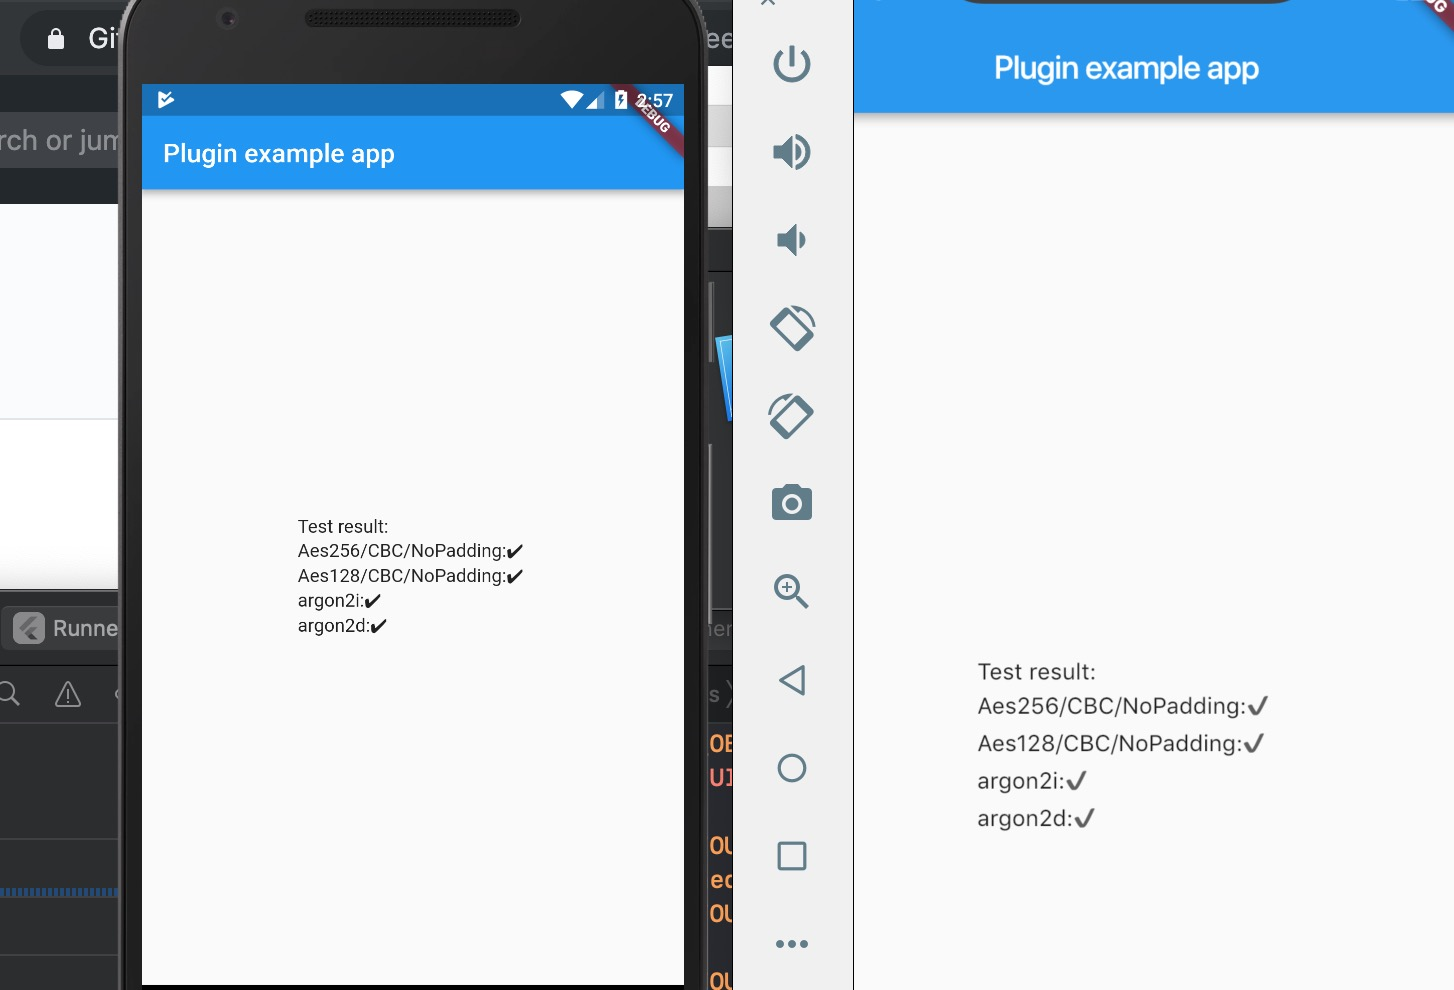
\includegraphics[keepaspectratio,alt={example}]{images/encryptions_example.jpeg}}
\caption{example}
\end{figure}

如果想了解更多，\href{https://github.com/soleverlee/encryptions}{这里}是详细的代码。

参考:

\begin{itemize}
\tightlist
\item
  \href{https://flutter.dev/docs/development/platform-integration/platform-channels}{Writing custom platform-specific code}
\item
  \href{https://flutter.dev/docs/development/packages-and-plugins/developing-packages}{Developing packages \& plugins}
\end{itemize}


\end{document}
